\section{Approach}
In the previous section we introduced IMCL's model approach to complex systems and the formal definition of the model. Based on this, we will introduce how to generate object code from the population IMCL model.

\begin{figure}[!htb]
  \centering
        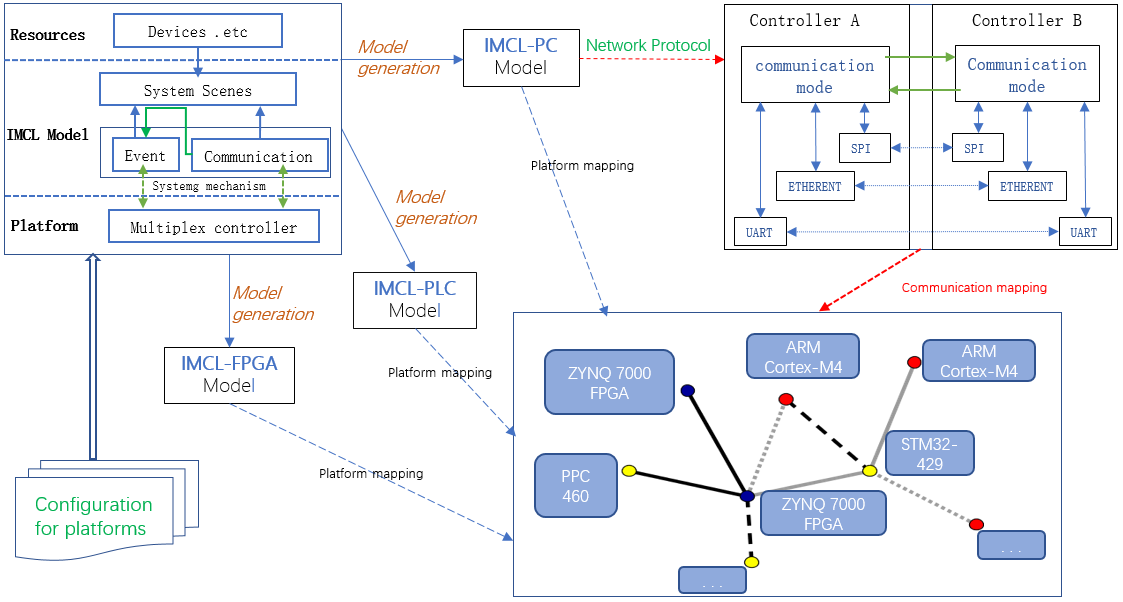
\includegraphics[height=1.4in, width=2.8in]{approach}
  \caption{The approach of IMCL Model to multi-platform code}\label{approach}
\end{figure}

The specific implementation details of the population model generation technique have been proposed in our previous published papers. The advantage of using the ICML modeling method is that we can intelligently split a complex model into multiple sub-models given the constraints of the resource and controller constraints. The sub-models can communicate with each other and achieve the same function as the original model. The generated sub-models correspond to specific target platforms respectively, and the main research work in this paper is to realize the code generation work from the IMCL model to different target platforms.


\subsection{Conversion of IMCL Model and Heterogeneous Platform}
We conduct research on different platforms, including FPGA, PLC, and PC. The research mainly includes how to use IMCL to represent these heterogeneous systems.

\subsubsection{\textbf{Conversion of FPGA and IMCL Model}}
FPGA (Field-Programmable Gate Array, Field Programmable Gate Array), due to its customizable features, is widely used in medical equipment, rail traffic control and other fields. The system developed by the VHDL language used by the FPGA includes the following basic parts:

\begin{itemize}
\item \textbf{Library} \ Declares the repository that the program needs to use, including the std, work, and user-defined libraries. Library contains a variety of design elements, from a program perspective, can be seen as a collection of data.
\item \textbf{Use} \ This section is related to the Library and declares the specific resources used by the corresponding resource library in the Library.
\item \textbf{Entity} \ This area is the entity declaration of the VHDL program and mainly describes the relationship between the input, output, and ports of the system circuit.
\item \textbf{Architecture} \ The architecture is the behavior part of the circuit. The architecture supports the parallel and serial of the program. The main description is its internal implementation process, including data flow, structure description, behavior description and so on.
\item \textbf{Configuration} \ The main purpose of the configuration is to select the required units from the library and form the required system. From the perspective of system resources, it is a process of choice and combination.
\end{itemize}

\begin{figure}[!htb]
  \centering
        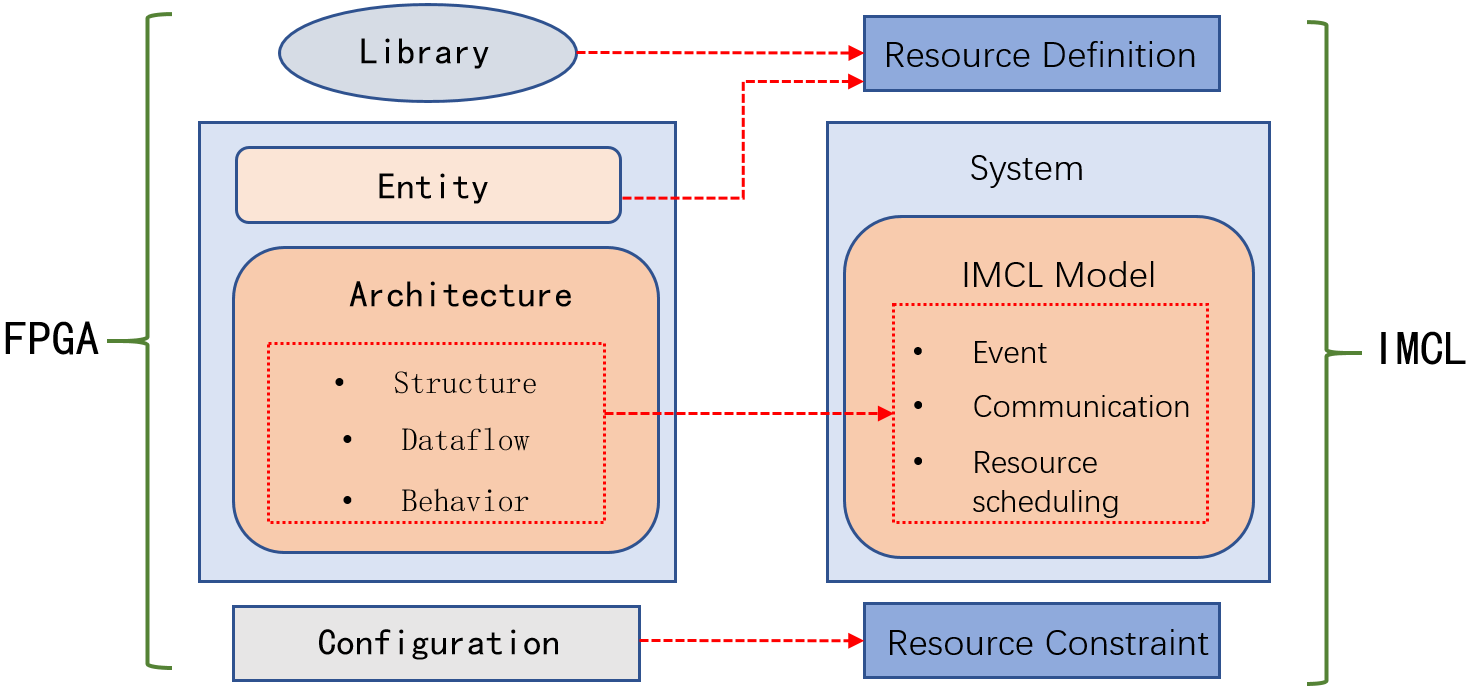
\includegraphics[height=1.4in, width=3.4in]{FPGA2IMCL}
  \caption{The transformation architecture of FPGA and IMCL-Model.}\label{FPGA2IMCL}
\end{figure}

Combined with the characteristics of the previously analyzed IMCL model, we can see that there are commonalities between the two architectures. After ignoring the irrelevant platform details, IMCL can model the behavior described by VHDL. As shown in the figure, the library and package structure represented in VHDL can be abstracted into resources in the process of modeling with IMCL after ignoring platform dependencies. The entity represents the design of the circuit structure of the system and can also be used as a description of resources. The architecture in VHDL mainly includes the structure description, data flow description, and system line description. Essentially, they describe the functional characteristics of the internal structure and correspond to the events described in IMCL.


\subsubsection{\textbf{Conversion of PLC and IMCL Model}}
PLC (Programmable Logic Controller) is a kind of programmable control industrial control computer. PLC takes the microprocessor as the core and realizes the control of the system through software. There are many types of PLCs, but their structural principles are basically the same: they include processors, storage, I/O ports, and network communications. Take the language IEC 61131-3 language by PLC as an example, the design language includes five forms: LD(Ladder Diagram),IL(Instruction List),FBD(Function Block Diagram),SFC(Sequential function chart),ST(Structured Text).

\begin{figure}[!htb]
  \centering
        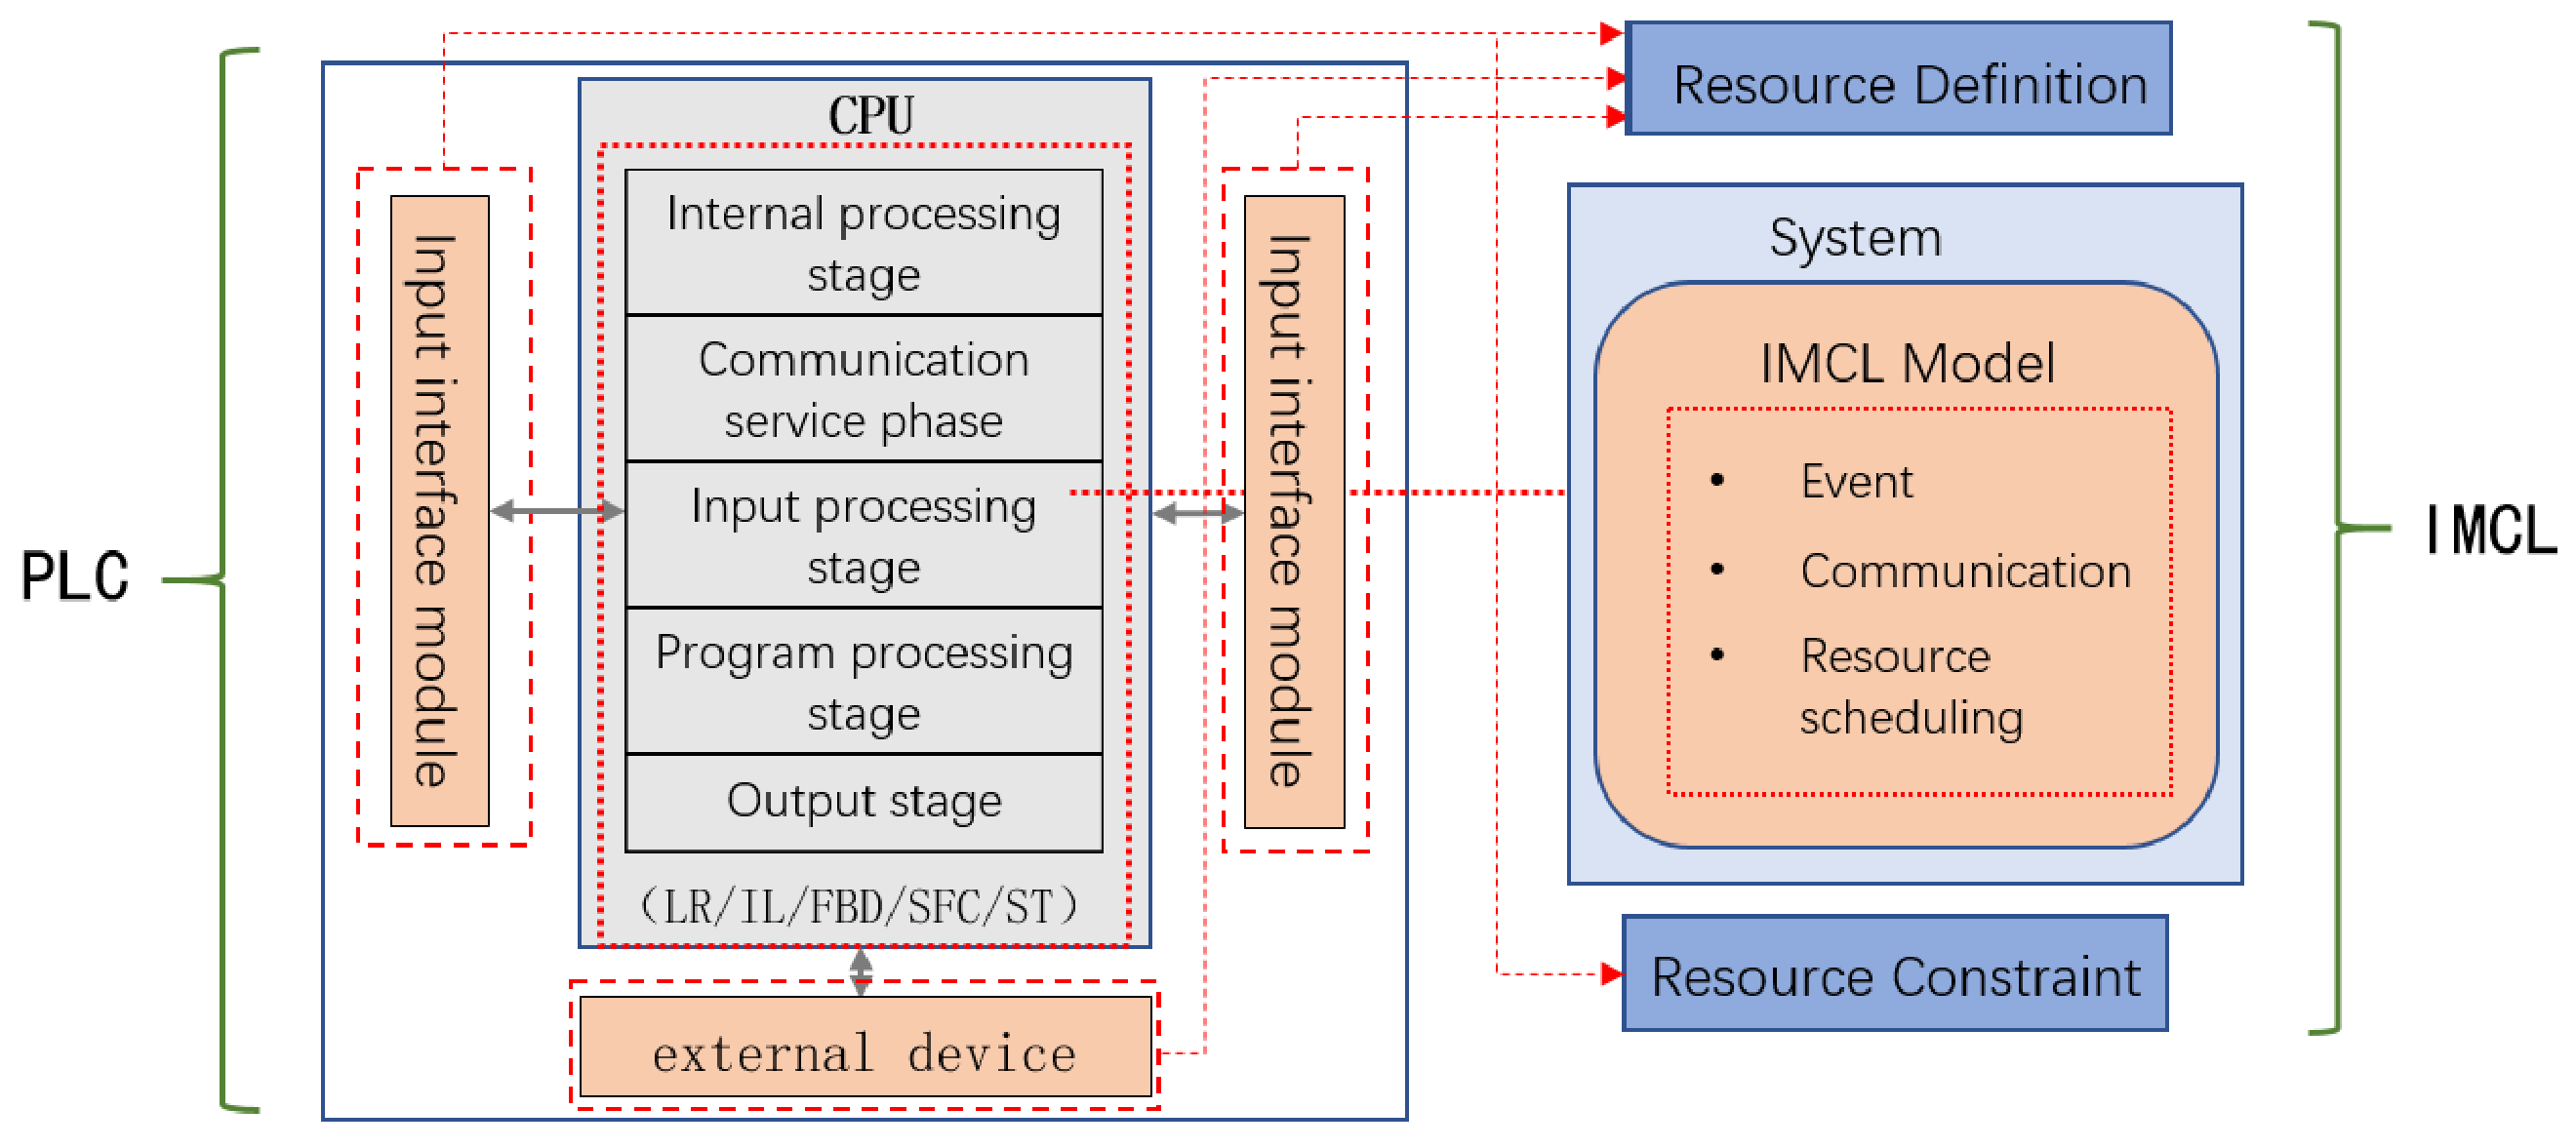
\includegraphics[height=1.4in, width=3.4in]{PLC2IMCL}
  \caption{The transformation architecture of PLC and IMCL-Model.}\label{PLC2IMCL}
\end{figure}

We can use IMCL to represent the operating mode of the PLC. The working phase of the PLC is to periodically scan cyclically, and it will continue to work when there is no interruption or other situations. The general PLC operating mode can be divided into five phases:

\begin{itemize}
  \item \textbf{Internal processing stage}: detecting the system's current ready state and resetting the internal timer;
  \item \textbf{Communication service phase}: The PLC has a communication function. The external control module can communicate with each other and can also receive signal commands from other controllers.
  \item \textbf{Input processing stage}: read the information data of the mounted peripherals and sample the data into the system at one time.
  \item \textbf{Program processing stage}: This stage is the core stage of the PLC control process and is the main body of the PLC program, including condition control, numerical calculation, and logic conversion. This stage reflects the functional behavior of the system.
  \item \textbf{Output stage}: After the main program runs, data is loaded to the outside through the output mechanism.
\end{itemize}

A unified description of the external physical resources associated with the input and output modules, peripherals, etc. The abstract resource object is a program variable, which can facilitate resource scheduling and set constraint conditions. For the main program of the PLC, we extract the main part of the communication services, program execution process, and then use an event-driven way to describe. Finally, the PLC application can be described by the IMCL model.

\subsubsection{Conversion of PC and IMCL Model}
PC (personal computer) is often widely applied to industrial systems because of its advantages such as high-speed processing speed, reliable operation platform, mass storage, networking, and friendly human-computer interaction. For example PCBCS, PC can communicate collaborate with other mainstream PC or PLC systems implement complex functional requirements. In PCBCS, PC's communication technology is one of its greatest advantages. PC can be compatible with almost all communication protocols in the mainstream, so it is very beneficial to the design of complex systems. The common PC system design language is C. Due to its good compatibility, portability, and high execution efficiency, it is widely used in industrial-grade system design.

\begin{figure}[!htb]
  \centering
        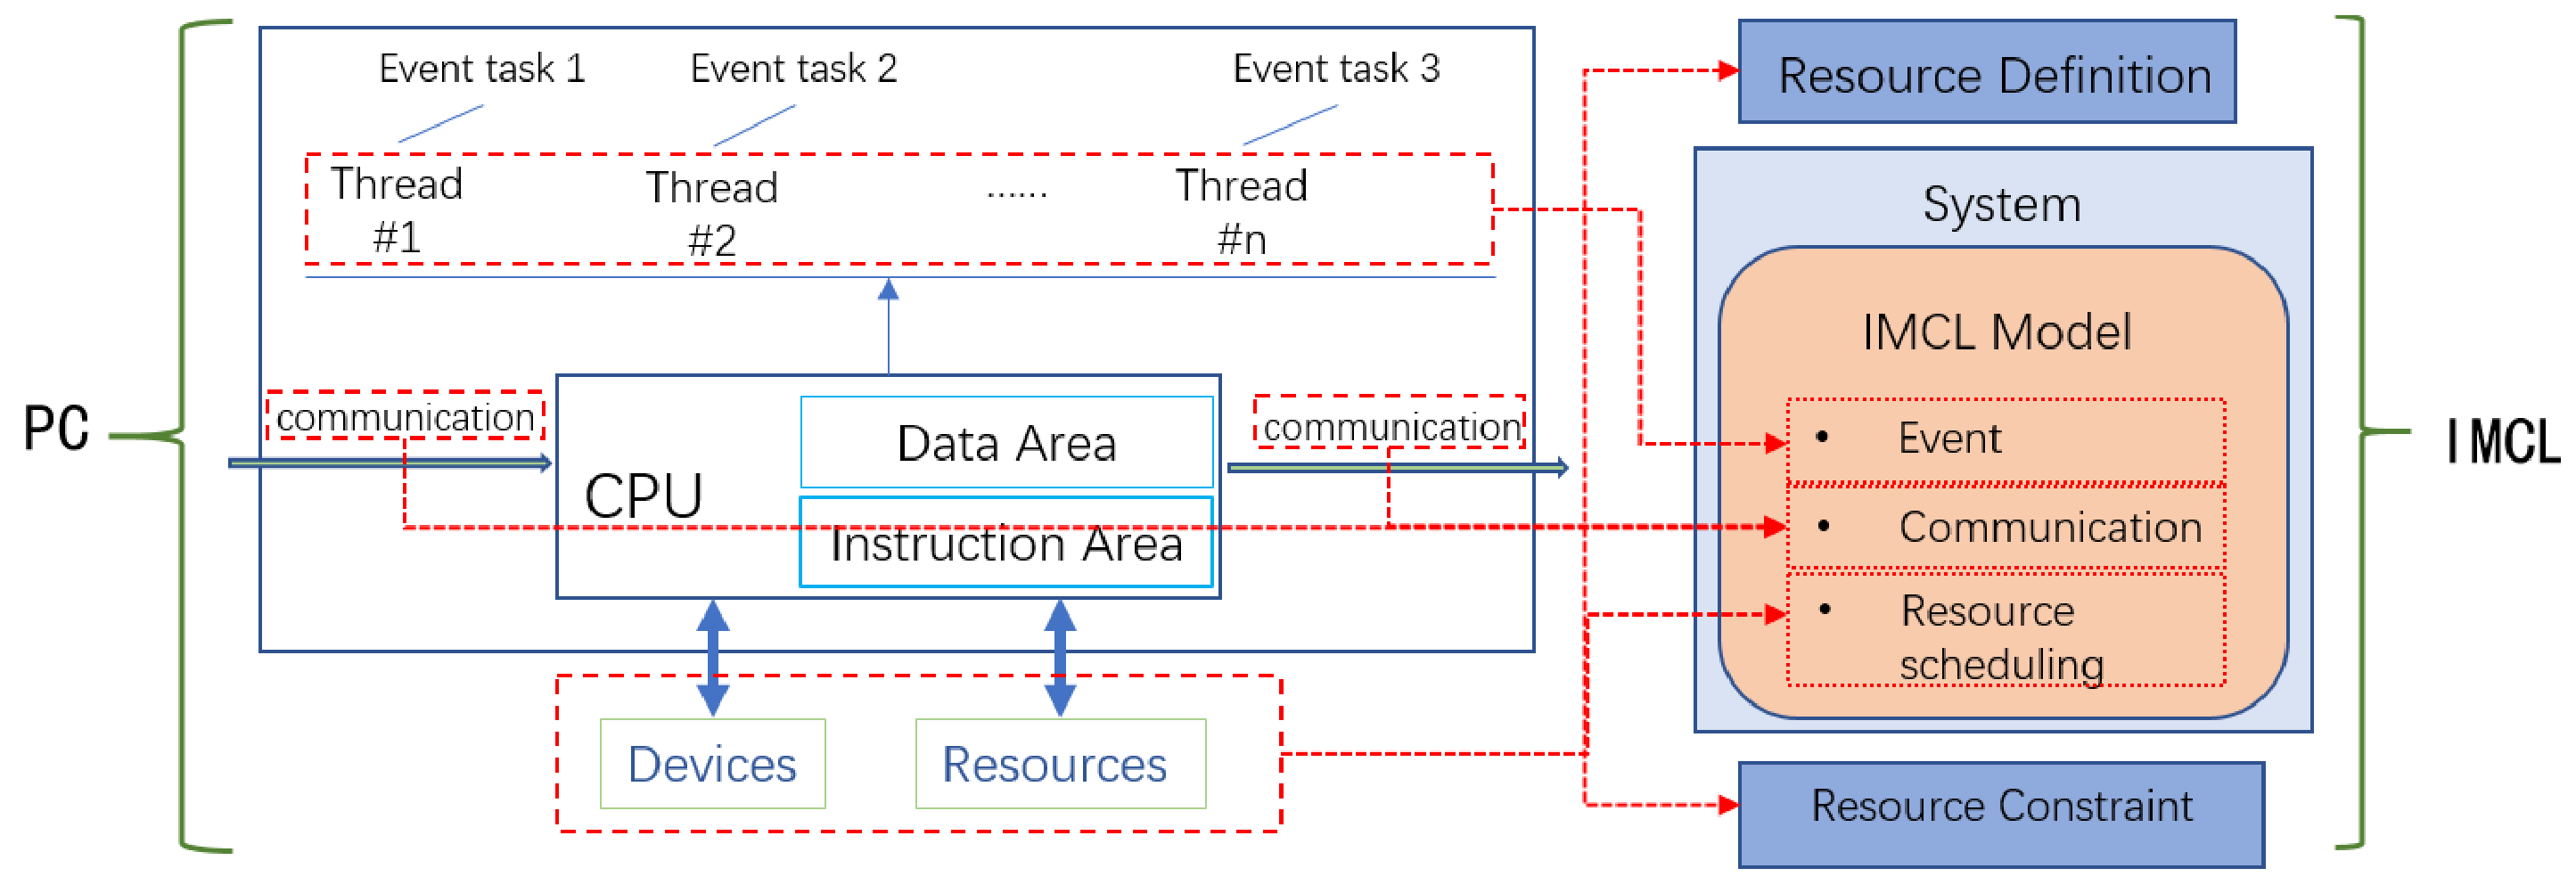
\includegraphics[height=1.4in, width=3.4in]{PC2IMCL}
  \caption{The transformation architecture of PC and IMCL-Model.}\label{PC2IMCL}
\end{figure}

As shown in the figure, a typical PC-style control system design can be represented as shown in the above figure. The CPU is responsible for the execution of the program. The entire system is composed of multiple independent threads. Each thread represents the relevant task. . The system has independent communication, including data input and output. When we use IMCL to model, we represent the multi-threading as a set of concurrent trigger events; the communication of system functions can be represented using the IMCL abstract communication protocol; the control relationship between the system and external device resources, using the resources in IMCL Scheduling to model.


\subsection{Code generation configuration}
The essence of the system model is to abstract away some irrelevant details and only pay attention to a research method to study the characteristics of the object. Therefore, when we want to be able to generate code from model automation, we need to supplement the missing details. In the code generation process from IMCL to a specific target platform, configuration information needed  includes variable conversion, communication protocol method between systems, and the driving relationship between a controller and specific devices. Here we use \emph{Conf} to represent these configuration: $Conf = \langle V_{map}, \ C_{map}, \ D_{map} \rangle$.

$V_{map}$ represents the variable mapping relationship between the model and the specified platform controller: $V_{map} = V_{imcl} \rightarrow (V_{plc} | V_{fpga}| V_{pc})$. The $V_{map}$ refers to the variables $V_{in} \cup V_{out} \cup V_{mess} \cup V_{local} \cup V_{res}$ in IMCL;  $V_{plc} | V_{fpga} | V_{pc}$ corresponds to a collection of variables for specific heterogeneous platforms.

$C_{map}$ represents the mapping relationship between the communication method in the model and the communication protocol used by a particular platform: $C_{map} = C_{imcl} \rightarrow (C_{plc} | C_{fpga} | C_{pc})$. $C_{imcl} = ch!Vmess | ch?V_{mess}$ refers to the formal representation of communications in IMCL; $C_{plc} | C_{fpga} | C_{pc}$ refers to the definition and implementation of specific communication protocols for different platforms.

$D_{map}$ represents the mapping relationship between the driver representation in the model and the drivers of controller and devices in  particular platforms: $D_{map} = D_{imcl} \rightarrow (D_{plc} | D_{fpga} | D_{soc})$.  $D_{imcl}=a_{data} \ll Dev | a_{data} \gg Dev$ refers to the scheduling relationship between the controller and peripheral physical devices in IMCL, and $(D_{plc} | D_{fpga} | D_{pc})$ corresponds to specific target platforms that need to implement the device scheduling driver. 